\documentclass[tikz,border=10pt]{standalone}
\usepackage{pgfplots}
\pgfplotsset{compat=1.18}
\usepackage{amsmath}
\usepackage{amssymb}
\definecolor{mantis}{RGB}{0, 105, 62}
\begin{document}
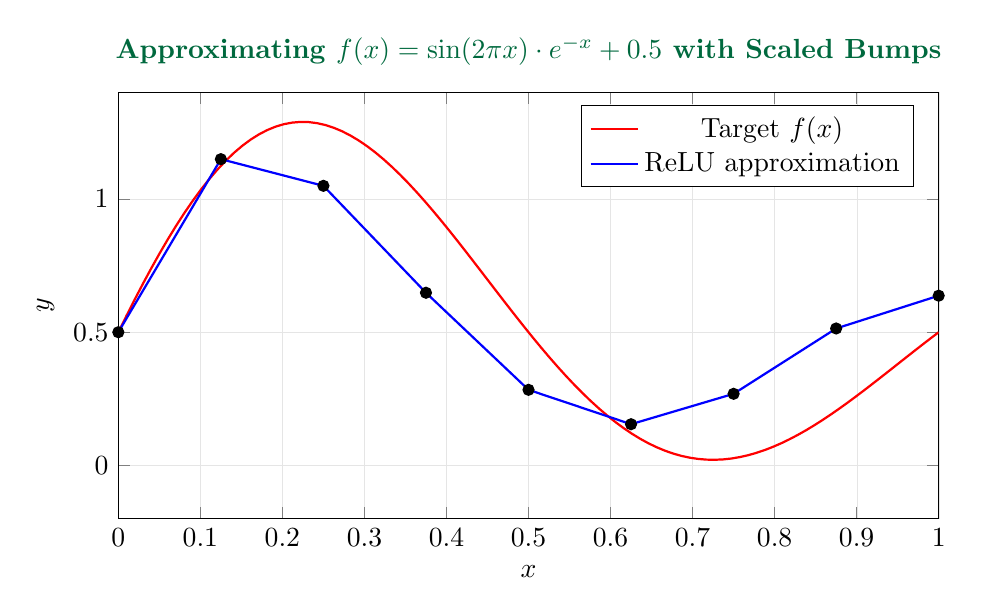
\begin{tikzpicture}
\begin{axis}[
    width=12cm,
    height=7cm,
    xlabel={$x$},
    ylabel={$y$},
    xmin=0, xmax=1,
    ymin=-0.2, ymax=1.4,
    title={\textbf{Approximating $f(x) = \sin(2\pi x) \cdot e^{-x} + 0.5$ with Scaled Bumps}},
    title style={font=\bfseries\color{mantis}},
    grid=both,
    grid style={line width=.1pt, draw=gray!20},
    legend pos=north east,
]
% Target function
\addplot[domain=0:1, samples=100, color=red, thick] {sin(deg(2*pi*x))*exp(-x) + 0.5};
\addlegendentry{Target $f(x)$}

% Bump approximation (piecewise linear)
\addplot[domain=0:0.125, samples=10, color=blue, thick] {0.5 + (0.5+0.649-0.5)/(0.125)*(x-0)};
\addplot[domain=0.125:0.25, samples=10, color=blue, thick] {0.5+0.649 + (0.5+0.549-0.5-0.649)/(0.125)*(x-0.125)};
\addplot[domain=0.25:0.375, samples=10, color=blue, thick] {0.5+0.549 + (0.5+0.148-0.5-0.549)/(0.125)*(x-0.25)};
\addplot[domain=0.375:0.5, samples=10, color=blue, thick] {0.5+0.148 + (0.5-0.216-0.5-0.148)/(0.125)*(x-0.375)};
\addplot[domain=0.5:0.625, samples=10, color=blue, thick] {0.5-0.216 + (0.5-0.345-0.5+0.216)/(0.125)*(x-0.5)};
\addplot[domain=0.625:0.75, samples=10, color=blue, thick] {0.5-0.345 + (0.5-0.231-0.5+0.345)/(0.125)*(x-0.625)};
\addplot[domain=0.75:0.875, samples=10, color=blue, thick] {0.5-0.231 + (0.5+0.014-0.5+0.231)/(0.125)*(x-0.75)};
\addplot[domain=0.875:1, samples=10, color=blue, thick] {0.5+0.014 + (0.5+0.137-0.5-0.014)/(0.125)*(x-0.875)};
\addlegendentry{ReLU approximation}

% Sample points
\addplot[only marks, mark=*, mark size=2pt, color=black] coordinates {
    (0, 0.5) (0.125, 1.149) (0.25, 1.049) (0.375, 0.648) (0.5, 0.284) (0.625, 0.155) (0.75, 0.269) (0.875, 0.514) (1, 0.637)
};
\end{axis}
\end{tikzpicture}
\end{document}
